\documentclass[12pt,national]{teaching}


\usepackage{fouriernc}
\usepackage[T1]{fontenc}

\begin{document}

\begin{comment}

\section*{Chimie}
\subsection*{Partie~1~: Cinétique chimique}
\begin{enumerate}
    \item Tableau d'avancement~:
          \begin{table}[H]
              \centering
              \renewcommand{\arraystretch}{1.5}
              \begin{tabularx}{\textwidth}{|p{2.5cm}|p{3.3cm}|p{3cm}|p{3cm}|X|X|}
                  \hline
                  \multicolumn{2}{|c}{Équation} &
                  \multicolumn{4}{|c|}{$\ce{2Fe^{2+}_{(aq)}}$ \qquad $+$ \qquad
                      $\ce{2Hg^{2+}_{(aq)}}$ \qquad
                      \ce{->} \qquad $\ce{2Fe^{3+}_{(aq)}}$ \qquad $+$ \qquad
                      $\ce{Hg^{2+}_{2}_{(aq)}}$} \\
                  \hline
                  État & Avancement~(mol) &
                  \multicolumn{4}{c|}{Quantités de matière (mol)}\\
                  \hline
                  initial & 0 & $n_{i}(\ce{Fe^{2+}})$ & $n_{i}(\ce{Hg^{2+}})$ &
                  $0$ & $0$ \\
                  \hline
                  intermédiaire & $x$ &
                  $n_{i}(\ce{Fe^{2+}})-2x$ & $n_{i}(\ce{Hg^{2+}})-2x$ &
                  $2x$ & $x$ \\
                  \hline
                  final & $x_{\max}$ &
                  $n_{i}(\ce{Fe^{2+}})-2x_{\max}$ &
                  $n_{i}(\ce{Hg^{2+}})-2x_{\max}$ &
                  $2x_{\max}$ & $x_{\max}$ \\
                  \hline
              \end{tabularx}
          \end{table}
          
          Déterminons l'avancement maximal $x_{\max}$~:
          \begin{itemize}
              \item Si \ce{Fe^{2+}} est le réactif limitant alors~: \\
                    $n_{i}(\ce{Fe^{2+}})-2x=0
                    \quad\Rightarrow x_{\max}=\frac{n_{i}(\ce{Fe^{2+}})}{2}=
                    \frac{[\ce{Fe^{2+}}]\cdot V}{2}
                    \quad\Rightarrow
                    x_{\max}=\frac{\num{1e-2}\times\num{100e-3}}{2}=
                    \qty{5e-4}{\mole}$.
              \item Si \ce{Hg^{2+}} est le réactif limitant alors~: \\
                    $n_{i}(\ce{Hg^{2+}})-2x=0
                    \quad\Rightarrow x_{\max}=\frac{n_{i}(\ce{Hg^{2+}})}{2}=
                    \frac{[\ce{Hg^{2+}}]\cdot V}{2}
                    \quad\Rightarrow
                    x_{\max}=\frac{\num{2e-2}\times\num{100e-3}}{2}=
                    \qty{1e-3}{\mole}$.
          \end{itemize}
          Donc le réactif limitant est \ce{Fe^{2+}} et l'avancement maximal
          vaut~: $\mathbox{x_{\max}=\qty{5e-4}{\mole}}$.

          \begin{minipage}[t][][t]{0.41\linewidth}
    \item On appelle temps de demi-réaction $t_{1/2}$ le temps nécessaire
          pour que l'avancement $x$ de la réaction soit égal à la moitié de
          sa valeur finale $x_{f}$~:
          \[
              x(t_{1/2})=\frac{x_{f}}{2}
          \]
          
          Dans notre cas, la réaction est totale,
          $x(t_{1/2})=\frac{x_{\max}}{2}$.

          Sur la courbe, on lit $\mathbox{t_{1/2}=\qty{14}{\hour}}$.
          \end{minipage}
          \hfill
          \begin{minipage}[t][][t]{0.55\linewidth}
              \begin{figure}[H]
              \centering
              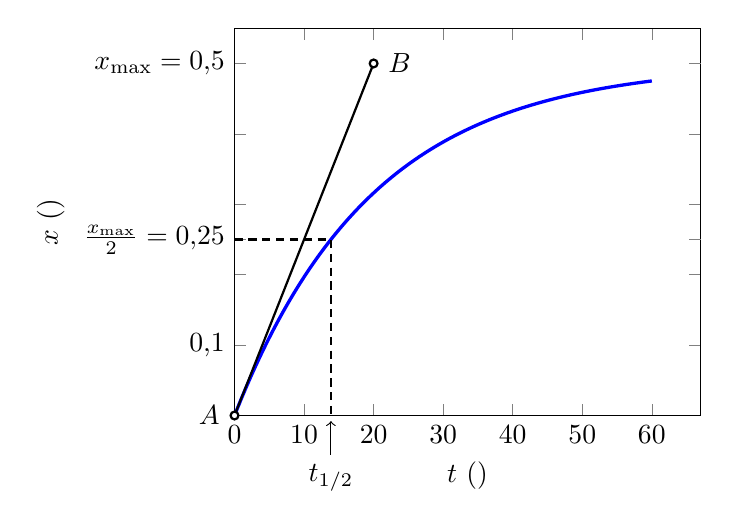
\begin{tikzpicture}
                  \def\xmax{0.5}
                  \def\k{0.05}
                  \pgfmathparse{ln(2)/\k}\let\tm=\pgfmathresult
                  \begin{axis}[
                          xmin=0, xmax=67,
                          ymin=0, ymax=0.55,
                          xtick distance=10,
                          ytick distance=0.1,
                          width=7.5cm, height=6.5cm,
                          xlabel=$t~(\unit{\hour})$,
                          ylabel=$x~(\unit{\mmol})$,
                          declare function={
                              droite0(\t)=\xmax*\k*\t;
                          },
                          %xticklabels={,,10},
                          yticklabels={,,{0,1}},
                          extra y ticks={0.25,0.5},
                          extra y tick labels={$\frac{x_{\max}}{2}=0{,}25$,
                            $x_{\max}=0{,}5$},
                      ]
                      \addplot[
                          domain=0:60,
                          samples=200,
                          blue,very thick,
                      ]
                      {\xmax*(1-exp(-\k*x))};
                      \draw[densely dashed,thick] (0,\xmax/2) -| (\tm,0)
                          coordinate(tm);
                      % droite
                      \addplot[
                          domain=0:20,
                          samples=100,
                          thick
                      ]
                      {droite0(x)}
                      coordinate[pos=0](A)
                      coordinate[pos=1](B);
                  \end{axis}
                  \draw[<-,shorten <=2pt] (tm) -- ++(0,-0.5)
                      node[below]{$t_{1/2}$};
                  \foreach \n/\a in {A/left,B/right}
                  \node[circle,draw,fill=white,thick,inner sep=1pt,
                      label=\a:$\n$] at (\n) {};
              \end{tikzpicture}
              \end{figure}
          \end{minipage}
    \item $v(t=0)=
          \frac{1}{V}\left.\frac{\mathrm{d} x}{\mathrm{d} t}\right|_{t=0}=
          \frac{1}{V}\left.\frac{\Delta x}{\Delta t}\right|_{t=0}=
          \frac{1}{V}\frac{x_{B}-x_{A}}{t_{B}-t_{A}}$ \\[2mm]
          $\Rightarrow v(t=0)=\frac{1}{\num{100e-3}}\frac{\num{0.5e-3}-0}{20-0}$
          $\Rightarrow \mathbox{v(t=0)=\qty{2.5e-4}{\mole\per\liter\per\hour}}$.

    \item La vitesse volumique de réaction \emph{diminue} au cours du temps.
          %Le facteur cinétique responsable de cette évolution est la
          %concentration des réactifs. En effet, cette concentration diminue au
          %cours du temps (car les réactifs sont consommées) et la vitesse de
          %réaction diminue aussi.
\end{enumerate}

\subsection*{Partie~2~: Acide monochloroéthanoïque}
\begin{enumerate}
    \item \textbf{Étude de la réaction entre l'acide monochloroéthanoïque et
          l'eau}
          \begin{enumerate}
              \item Un acide selon Brönsted est une espèce chimique capable de
                    \emph{fournir} un proton \ce{H+}.
              \item 
                    \begin{enumerate}
                        \item 
                    Tableau d'avancement~:
                    \begin{table}[H]
                        \centering
                        \renewcommand{\arraystretch}{1.5}
                        \begin{tabularx}{\textwidth}{|p{2.5cm}|p{3.3cm}|p{3cm}|p{3cm}|X|X|}
                            \hline
                            \multicolumn{2}{|c}{Équation} &
                            \multicolumn{4}{|c|}{$\ce{AH_{(aq)}}$
                                \qquad $+$ \qquad
                                $\ce{H2O_{(\ell)}}$ \qquad
                                \ce{<=>} \qquad $\ce{A^-_{(aq)}}$
                                \qquad $+$ \qquad
                                $\ce{H3O^{+}_{(aq)}}$} \\
                            \hline
                            État & Avancement~(mol) &
                            \multicolumn{4}{c|}{Quantités de matière (mol)}\\
                            \hline
                            Initial & 0 & $n_{i}(\ce{AH})$ & excès &
                            $0$ & $0$ \\
                            \hline
                            Intermédiaire & $x$ &
                            $n_{i}(\ce{AH})-x$ & excès &
                            $x$ & $x$ \\
                            \hline
                            Équilibre & $x_{\eq}$ &
                            $n_{i}(\ce{AH})-x_{\eq}$ &
                            excès &
                            $x_{\eq}$ & $x_{\eq}$ \\
                            \hline
                        \end{tabularx}
                    \end{table}
              \item On a~: $\sigma=\sum_{i}\lambda_{i}\cdot[X_{i}]$.
                    Les ions présents dans la solutions sont~: \ce{A-} et
                    \ce{H3O+}. Donc~: \\
                    $\sigma=\lambda_{\ce{H3O+}}\cdot[\ce{H3O+}]+
                    \lambda_{\ce{A-}}\cdot[\ce{A-}]$.

                    D'après le tableau,
                    $[\ce{H3O+}]=[\ce{A-}]=\frac{x_{\eq}}{V}$. D'où~:
                    $\sigma=(\lambda_{1}+\lambda_{2})\cdot\frac{x_{\eq}}{V}$.
                    Ce qui donne~:

                    \begin{minipage}[t][][t]{0.64\linewidth}
                        \[
                            \mathbox{x_{\eq}=
                            \frac{\sigma\cdot V}{\lambda_{1}+\lambda_{2}}}
                        \]
                        A.N. $x_{\eq}=\frac{0,3\times\num{100e-3}\times\num{1e-3}}
                        {\num{35e-3}+\num{4e-3}}$
                        \quad
                        $\Rightarrow\mathbox{x_{\eq}\simeq\qty{7.7e-4}{\mole}}$.
                    \end{minipage}
                    \hfill
                    \begin{minipage}[t][][b]{0.35\linewidth}
                        \flushright
                        \begin{tcolorbox}[enhanced,size=small,drop fuzzy shadow,
                            sharp corners,colframe=cadmiumred,
                            title={\faBomb\; Attention},
                            fonttitle=\bfseries]
                            $\sigma$ est en $\unit{\siemens\per\meter}$,
                            donc $V$ est en $\unit{\cubic\meter}$.\\
                            $\qty{1}{\L}=\qty{1e-3}{\cubic\meter}$.
                        \end{tcolorbox}
                    \end{minipage}
                        \item On a~: $\tau=\frac{x_{\eq}}{x_{\max}}$.
                              Déterminons l'avancement maximal $x_{\max}$~:
                              l'eau est en excès alors le réactif limitant est
                              \ce{AH}. Donc~: $n_{i}(\ce{AH})-x_{\max}=0$ soit
                              $x_{\max}=n_{i}(\ce{AH})=\qty{5e-3}{\mole}$.

                              D'où~:
                              $\tau=\frac{\num{7.7e-4}}{\num{5e-3}}$
                              \quad $\Rightarrow
                              \mathbox{\tau=\qty{0.154}{\mole}}$.
                    \end{enumerate}
              \item $\mathrm{K_{A}}=\frac{[\ce{A-}]_{\eq}\cdot[\ce{H3O+}]_{\eq}}
                    {[\ce{AH}]_{\eq}}=\frac{\left(\frac{x_{\eq}}{V}\right)^{2}}
                    {\left(\frac{n_{i}(\ce{AH})-x_{\eq}}{V}\right)}=
                    \frac{x_{\eq}^{2}}
                    {V\cdot\left(n_{i}(\ce{AH})-x_{\eq}\right)}$

                    Or, $\tau=\frac{x_{\eq}}{x_{\max}}=
                    \frac{x_{\eq}}{n_{i}(\ce{AH})}$ \quad
                    $\Rightarrow x_{\eq}=\tau\cdot n_{i}(\ce{AH})$.
                    En remplaçant dans $\mathrm{K}_{A}$, on obtient~: \\
                    $\mathrm{K_{A}}=
                    \frac{\left(\tau\cdot n_{i}(\ce{AH})\right)^{2}}{V\cdot
                    \left(n_{i}(\ce{AH})-\tau\cdot n_{i}(\ce{AH})\right)}$.
                    D'où~:
                    $\mathbox{\mathrm{K_{A}}=
                    \frac{\tau^{2}\cdot n_{i}(\ce{AH})}{V\cdot(1-\tau)}}$.
              \item A.N. 
                    $\mathrm{K_{A}}=\frac{(0,154)^{2}\times\num{5e-3}}
                    {\num{100e-3}\times(1-0,154)}$ \quad
                    $\Rightarrow\mathbox{\mathrm{K_{A}}=\num{1.4e-3}}$.
          \end{enumerate}
    \item \textbf{Détermination de la concentration d’acide
          monochloroéthanoïque dans un médicament}
          \begin{enumerate}
              \item $\ce{AH_{(aq)} + HO^-_{(aq)} -> A^-_{(aq)} + H2O_{(\ell)}}$.
              \item Relation d'équivalence~:
                    $C_{1}V_{1}=C_{B}V_{B,E}$, donc~:
                    $C_{1}=\frac{C_{0}}{10}=\frac{C_{B}V_{B,E}}{V_{1}}$ \quad
                    $\Rightarrow C_{0}=\frac{10\cdot C_{B}\cdot
                    V_{B,E}}{V_{1}}$.

                    A.N. $C_{0}=\frac{10\times0,10\times 21}{10}$ \quad
                    $\Rightarrow \mathbox{C_{0}=\qty{2.1}{\M}}$.
          \end{enumerate}
\end{enumerate}


\section*{Physique}
\subsection*{Exercice~1}
\begin{enumerate}
    \item
          \begin{enumerate}
              \item Une onde mécanique progressive périodique est dite
                    sinusoïdale si l'évolution temporelle de la source peut être
                    associée à une fonction sinusoïdale.
              \item L'onde est \emph{transversale}, car la direction de la
                    perturbation du milieu est perpendiculaire à la direction de
                    propagation.
          \end{enumerate}
    \item \mbox{}\par
          \begin{minipage}[t][][t]{0.65\linewidth}
              \begin{enumerate}
                  \item $\lambda=\qty{2}{\cm}$.
                  \item On a~: $v=\lambda \cdot N$ \quad
                        A.N. $v=\num{2e-2}\times 20$
                        \quad $\Rightarrow \mathbox{v=\qty{0.4}{\v}}$.
                  \item On a~:
                        $v=\frac{d}{\Delta t}=\frac{d}{t_{1}-t_{0}}=
                        \frac{d}{t_{1}}$ \quad $\Rightarrow t_{1}=\frac{d}{v}$ 
                        
                        A.N. $t_{1}=\frac{\num{4e-2}}{0,4}$
                        \quad $\Rightarrow \mathbox{t_{1}=\qty{0.1}{\s}}$.
              \end{enumerate}
          \end{minipage}
          \hfill
          \begin{minipage}[t][][t]{0.34\linewidth}
              \begin{figure}[H]
                  \centering
                  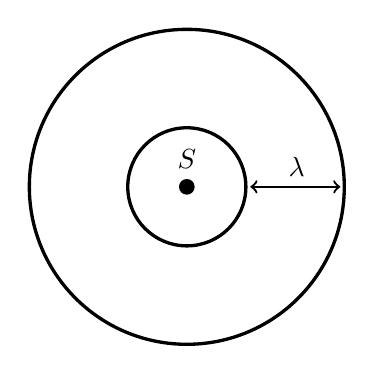
\begin{tikzpicture}
                      \node[circle,draw,very thick,minimum size=1.5cm] (C1) {};
                      \node[circle,draw,very thick,minimum size=4cm] (C2) {};
                      \node[circle,fill,inner sep=2pt,label=$S$] (O) {};
                      \draw[<->,shorten <=1pt,shorten >=2pt,thick]
                          (C1.east) -- (C2.east)
                          node[above,pos=0.5] {$\lambda$};
                  \end{tikzpicture}
              \end{figure}
          \end{minipage}
    \item $y_{M}(t)=y_{S}(t-\tau)$ \quad avec
          $\tau=\frac{SM}{v}=\frac{d}{v}=t_{1}=\qty{0.1}{\s}$.
          Donc~: $\mathbox{y_{M}(t)=y_{S}(t-0,1)}$.
    \item On a~: $v^{\prime}=\lambda^{\prime} \cdot N^{\prime}$ \quad
          A.N. $v^{\prime}=\num{3e-2}\times 10$
          \quad $\Rightarrow \mathbox{v^{\prime}=\qty{0.3}{\v}}$.

          $v^{\prime} \neq v$, la vitesse de l'onde dans ce milieu dépend de sa
          fréquence. Le milieu est \emph{dispersif}.
    \item 
          \begin{minipage}[t][][t]{0.55\linewidth}
              \begin{enumerate}
                  \item $\lambda=\qty{2}{\cm}$ et $a=\qty{0.5}{\cm}$. Or
                        $a<\lambda$, une phénomène de \emph{diffraction} se
                        produira.
                  \item 
                        \begin{itemize}
                            \item L'onde diffractée est circulaire.
                            \item Les deux ondes incidentes et diffractée ont
                                  même fréquence $N$, même vitesse $v$ et même
                                  longueur d'onde $\lambda$.
                        \end{itemize}
              \end{enumerate}
          \end{minipage}
          \hfill
          \begin{minipage}[t][][t]{0.44\linewidth}
              \begin{figure}[H]
                  \centering
                  \begin{tikzpicture}
                      \newdimen\h \h=3.5cm
                      \newdimen\la \la=5mm
                      \newdimen\a \a=3mm
                      \node[fill,inner sep=0pt,minimum width=5pt,
                          minimum height=\h] (P) {};
                      \node[fill=white,inner sep=0pt,minimum width=6pt,
                          minimum height=\a] (F) at (P.center) {};
                      \draw[{Stealth[length=4pt]}-{Stealth[length=4pt]},
                          thick] (F.north west) --
                          node[left=-1mm] {$a$} (F.south west);
                      \foreach \x [count=\i] in {-3,-2.5,...,-0.5}
                      \node[fill=blue,inner sep=0pt,minimum width=1.2pt,
                          minimum height=\h] (p\i) at (\x,0) {};
                      \draw[<->,shorten <=0.4pt,shorten >=0.4pt]
                          (p3) -- (p4) node[above,pos=0.5] {$\lambda$};
                      \coordinate (S) at ([xshift=3pt]F.center);
                      \foreach \r [count=\i] in {0.4,0.9,...,3}
                      \draw[line width=1.2pt,blue]
                          ([shift=(-40:\r cm)]S) arc (-40:40:\r cm);
                      \draw[<->,shorten <=0.6pt,shorten >=0.6pt]
                          ([xshift=2cm]F.center) -- ++(0.5,0)
                          node[above,pos=0.5] {$\lambda$};
                  \end{tikzpicture}
              \end{figure}
          \end{minipage}
\end{enumerate}

\end{comment}

\subsection*{Exercice~3}
\subsubsection*{Partie~1~: Élude du mouvement d'une bille en chute libre}

\begin{enumerate}
    \item
          \begin{minipage}[t][][t]{0.58\linewidth}
          \begin{itemize}
              \item \textbf{Système étudié~:} la bille de masse $m$.
              \item \textbf{Force exercée sur la bille~:} le poids $\vec{P}$.
              \item \textbf{Application de la deuxième loi de Newton~:} \par
                    $\sum \vec{F}_{\text{ext}}=m \vec{a}_G
                    \;\Rightarrow \vec{P}=m \vec{a}_G \;\Rightarrow m \vec{g}=m
                    \vec{a}_G$, donc~:
                    \begin{equation}
                        \mathbox{\vec{a}_G=\vec{g}}\label{eq:diff}
                    \end{equation}
                    On projette l'équation~\ref{eq:diff} sur l'axe $(Oz)$,
                    on obtient~: $a_{z}=g$.
                    \[
                        \Rightarrow\mathbox{%
                        \frac{\mathrm{d}^{2} z_{G}}{\mathrm{d} t^{2}}=g}
                        \quad\text{(équation différentielle)}
                    \]
          \end{itemize}
          \end{minipage}
          \hfill
          \begin{minipage}[t][][t]{0.40\linewidth}
          \begin{figure}[H]
              \flushright
              \begin{tikzpicture}
                  \newdimen\h \h=3.4cm
                  \draw[-Latex,shorten <=-0.8\h]
                      (0,0) coordinate(O) -- ++(0,-1.2\h)
                      node[left] {$z$};
                  \draw[->,thick] (O) -- ++(0,-1)
                      node[left,pos=0.8] {$\vec{k}$};
                  \node[circle,ball color=lightgray,draw,densely dashed,
                      inner sep=5pt] (S) at (1,0) {};
                  \node[circle,inner sep=1pt,fill,
                      label={[above left=1mm]:$A$}] (A) at (S.center) {};
                  \node[circle,ball color=lightgray,draw,
                      inner sep=5pt] (S2) at (1,0.67\h) {};
                  \node[circle,inner sep=1pt,fill] (B) at (S2.center) {};
                  \draw[->,line width=0.6pt]
                      (A) -- ++(0,0.7) node[right,pos=0.75] {$\vec{V}_{0}$};
                  \draw[dashed] (O) -- (A) (B) -- (B -| O);
                  \node[fill,minimum width=1.5cm,anchor=north,inner sep=3pt,
                      label=right:sol] (sol) at ([yshift=-\h]A) {};
                  \foreach \y/\n in {0/O,-\h/h,0.67\h/z_{1}}
                      \draw[thick] (3pt,\y) -- (-3pt,\y)
                          node[left] {$\n$};
                  % 
                  \draw[->,line width=0.8pt,red]
                      (A) -- ++(0,-1.3) node[right,pos=0.8] {$\vec{P}$};
                  %
                  \foreach \b/\t/\v in {S/0/V_{0},S2/t_{1}/0}
                      \node[right=3mm] at (\b.east) {à $t=\t$, $v_{G}=\v$};
                  \draw[{Bar[].Stealth[]}-{Stealth[].Bar[]},thick]
                      ([xshift=-1.4cm]sol.north west) coordinate(tmp) --
                      (tmp |- B) node[pos=0.5,left] {$h_{m}$};
              \end{tikzpicture}
              \caption{}
              \label{fig:bille}
          \end{figure}
          \end{minipage}

    \item On a~: $\vec{a}=\vv{\mathrm{cte}}$, donc le mouvement de chute libre
          de la bille est \emph{rectiligne uniformément varié}.
    \item 
          \begin{enumerate}
              \item $G$ atteint la hauteur maximale lorsque $v_{G}=0$. Donc~:
                    $10t_{1}-4=0$ \quad $\Rightarrow t_{1}=\frac{4}{10}$ 
                    \quad $\Rightarrow\mathbox{t_{1}=\qty{0.4}{\second}}$.
              \item On a~: $v_{G}=\frac{\mathrm{d} z_{G}}{\mathrm{d} t}=10t-4$.
                    On intègre cette équation, on obtient~:
                    $z_{G}(t)=\frac{1}{2}\cdot 10\cdot t^{2}-4\cdot t+C$, avec
                    $C$ est une constante à déterminée par les conditions
                    initiales.

                    D'après les données du problème, à $t=0$, $z_{G}=z_{A}=0$.
                    Donc~: \\
                    $z_{G}(t=0)=5\times 0^{2}-4\times 0+C=0$ \quad
                    $\Rightarrow C=0$.

                    L'équation horaire est données par~:
                    \[
                        z_{G}(t)=5 t^{2}-4 t.
                    \]
                    $G$ atteint la hauteur maximale $h_{m}$ lorsque $t=t_{1}$.
                    Donc~: \\
                    $z_{G}(t_{1})=z_{1}=5 t_{1}^{2}-4 t_{1}=
                    4\times0,4-4\times0,4$ \quad
                    $\Rightarrow z_{1}=-\qty{0,8}{\meter}$.

                    D'où~: $h_{m}=h+|z_{1}|=1,2+0,8$ \quad
                    $\Rightarrow \mathbox{h_{m}=\qty{2}{\meter}}$
          \end{enumerate}
\end{enumerate}

\subsubsection*{Partie~2~: Étude du mouvement de l'oscillateur
\{solide - ressort\}}
\begin{enumerate}
    \item Graphiquement~: $\mathbox{X_{m}=\qty{4}{\cm}}$ et
          $\mathbox{T_{0}=\qty{0.5}{\second}}$.
    \item On a~: $T_{0}=2\pi\sqrt{\frac{m}{K}}$, donc~:
          $K=\frac{4\pi^{2}m}{T_{0}^{2}}$. 
          A.N. $K=\frac{4\pi^{2}\times\num{125e-3}}{0,5^{2}}$ \quad
          $\Rightarrow \mathbox{K=\qty{19.7}{\newton\per\meter}}$
    \item On a~: $\vec{F}=-Kx\ex$, donc~:
          $F=K|x|=KX_{m}\left|\cos\left(\frac{2\pi}{T_{0}}t\right)\right|$.

          À $t_{1}=\frac{5}{2}T_{0}$, 
          $F_{1}=KX_{m}\left|\cos\left(\frac{2\pi}{T_{0}}t_{1}\right)\right|=
          KX_{m}\left|\cos\left(\frac{2\pi}{T_{0}}\cdot\frac{5}{2}T_{0}\right)
          \right|=KX_{m}\left|\cos(5\pi)\right|=KX_{m}$ \\
          A.N. $F_{1}=19,7\times\num{4e-3}$ \quad
          $\Rightarrow \mathbox{F_{1}=\qty{0.79}{\newton}}$
\end{enumerate}

\end{document}
